% Telekom osCompendium 'for beeing included' snippet template
%
% (c) Karsten Reincke, Deutsche Telekom AG, Darmstadt 2011
%
% This LaTeX-File is licensed under the Creative Commons Attribution-ShareAlike
% 3.0 Germany License (http://creativecommons.org/licenses/by-sa/3.0/de/): Feel
% free 'to share (to copy, distribute and transmit)' or 'to remix (to adapt)'
% it, if you '... distribute the resulting work under the same or similar
% license to this one' and if you respect how 'you must attribute the work in
% the manner specified by the author ...':
%
% In an internet based reuse please link the reused parts to www.telekom.com and
% mention the original authors and Deutsche Telekom AG in a suitable manner. In
% a paper-like reuse please insert a short hint to www.telekom.com and to the
% original authors and Deutsche Telekom AG into your preface. For normal
% quotations please use the scientific standard to cite.
%
% [ Framework derived from 'mind your Scholar Research Framework' 
%   mycsrf (c) K. Reincke 2012 CC BY 3.0  http://mycsrf.fodina.de/ ]
%


%% use all entries of the bibliography
%\nocite{*}

[TDB \ldots]

Be careful: Linux Magazine (04/05 2011) uses another taxonomy which seems not
to be as elaborated as this taxonomy. This must be discussed[\ldots]
\ldots

\section{Minimal Prescribing Licensemodels: Protecting the developer}
\footnotesize
\begin{quote}\itshape
Here we discuss licenses which only try to protect the developer, like
the licenses \emph{BSD}, \emph{MIT} and \emph{Apache}.
\end{quote}
\normalsize
\ldots

\section{Reflexive Prescribing Licensemodels: Protecting the code}
\footnotesize
\begin{quote}\itshape
Here we discuss licenses which try to protect the developer and to protect the
licensed code, like the licenses \emph{EPL?}, \emph{EUPL?} and
\emph{LGPL}
\end{quote}
\normalsize
\ldots

\section{Overlapping Prescribing Licensemodels: Protecting the on-top-developments}
\footnotesize
\begin{quote}\itshape
Here we discuss licenses which try to protect the developer, which try to
protect the licensed code, and which try to protect the on-top-developments,
also known as derivated works. You may expect the licenses \emph{GPL-2},
\emph{GPL-3}, and \emph{AGPL}\ldots
\end{quote}
\normalsize
\ldots

\subsection{Excursion: GPL is not the Evil}
\footnotesize
\begin{quote}\itshape
Here we simply want to underline that licenses protecting the
on-top-developments does not 'infect' other proprietary software automatically.
It's not an aspect of the code of the license, but of the acts of the combining
developers or managers. It's their decision if they have to fulfill the GPL.
\end{quote}
\normalsize
\ldots

\subsection{Excursion: The Peculiarity of GPL-3}
\footnotesize
\begin{quote}\itshape
In the same sense we want to explain how the GPL-3 only upholdes former ideas by
transposing them to new technical trends.
\end{quote}
\normalsize
\ldots

\section{Other Models}
\ldots Do they exist? \ldots

\section{Summary: Our Taxonomy for the analyzed Licenses}
\footnotesize
\begin{quote}\itshape
One pictures and the hint, that the criteria can be implemented differently by
diffrent licenses and that one therefore has to analyze the single licenses
nevertheless.
\end{quote}
\normalsize
\ldots

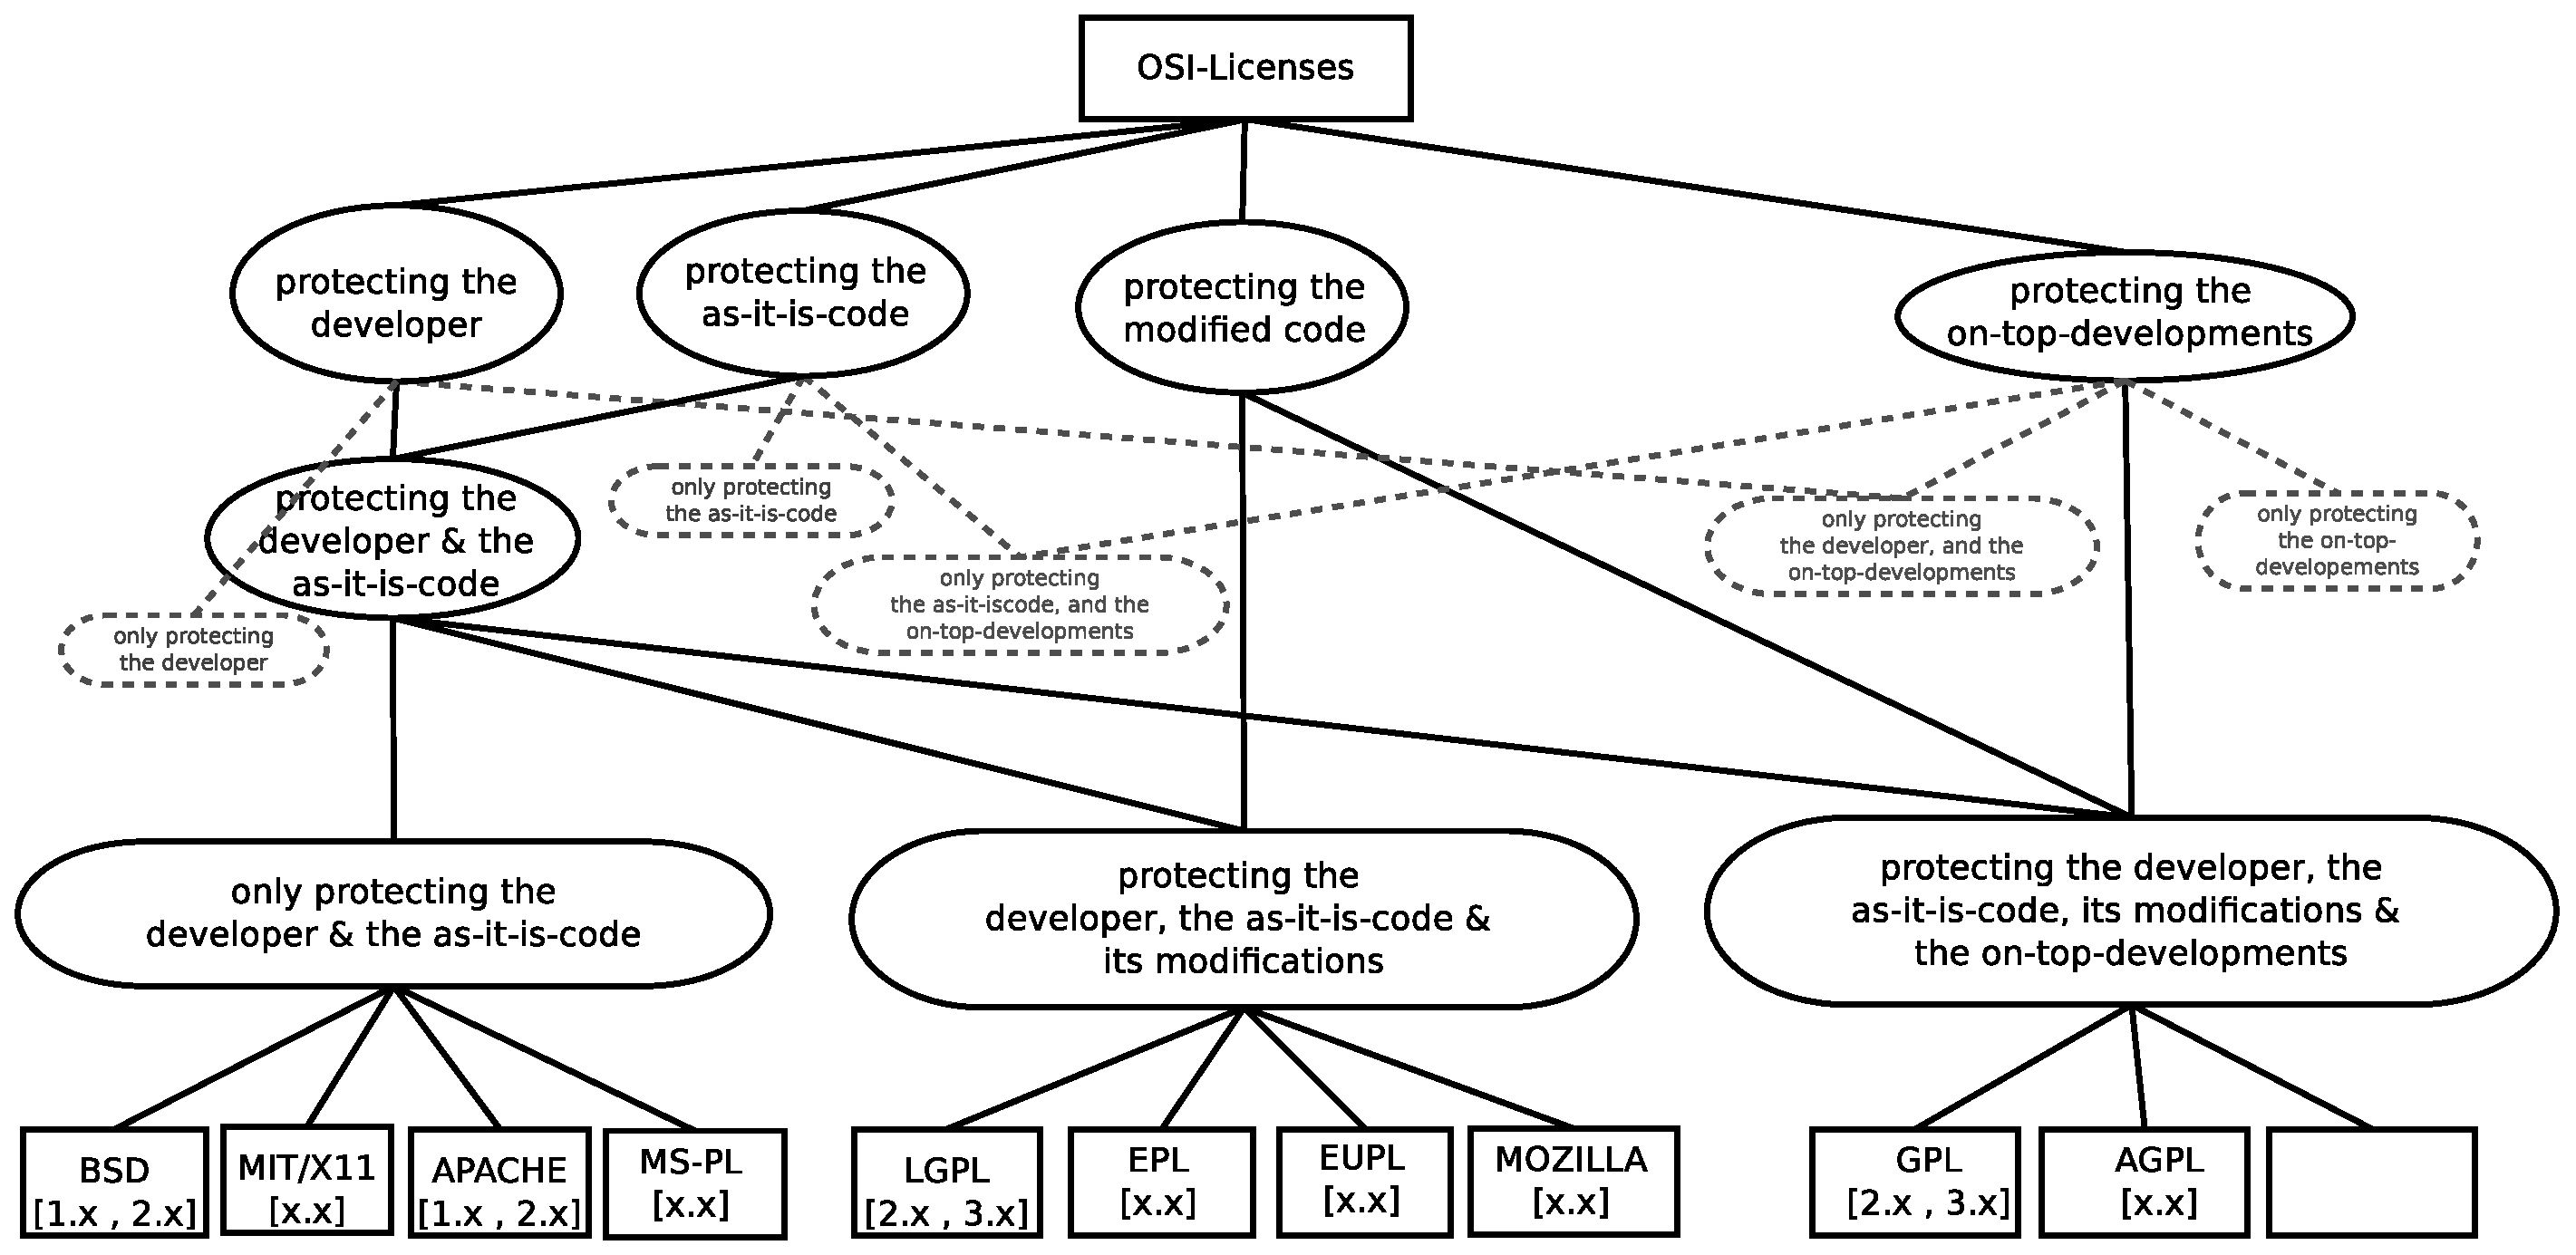
\includegraphics[scale=0.32]{graphics/licenses-cluster.eps}


%\bibliography{../../../bibfiles/oscResourcesEn}
